\documentclass[12pt]{article}
\newif\ifanswer\answertrue\answerfalse% comment out to show/hide answers
\usepackage{../preamble3}% preamble always after \newif\ifanswer
%\pagenumbering{gobble}
\title{Art Of Problem Solving - AMC 10 \\ Week 5}
\author{Patrick \& James Toche}
\date{July 10, 2021}

\begin{document}
\maketitle
\begin{minipage}{\textwidth}
\begin{abstract}\setlength{\parindent}{0pt}%
Notes on the AMC-10 Course by Art Of Problem Solving (AOPS).
Copyright restrictions may apply. Written for personal use. 
Please report typos and errors over at \url{https://github.com/ptoche/Math/tree/master/aops}. 
\end{abstract}
\end{minipage}

\thispagestyle{empty}
\clearpage


%%%%%%%%%%%%%%%%%%%%%%%%%%%%%%%%%%%%%%%%%%%%%%%%%%%%%%%%%%%%%%%%%%%%%%%%
\subsection*{1.}

\nopagebreak

In a collection of red, blue, and green marbles, there are $25\%$ more red marbles than blue marbles, and there are $60\%$ more green marbles than red marbles. Suppose that there are $r$ red marbles. What is the total number of marbles in the collection?

\nopagebreak

\fbox{(A) $2.85r$ \quad (B) $3r$ \quad (C) $3.4r$ \quad (D) $3.85r$ \quad (E) $4.25r$}

\begin{answer}
Let $r$, $b$, $g$ denote the number of red, blue, green marbles, where $r$ is given. The total number is $r+b+g$. The  stated conditions are:
\begin{align*}
r & = 1.25b \\
g & = 1.6 r
\end{align*}
This gives the sum:
\begin{align*}
r + b + g 
  & = r + \frac{r}{1.25} + 1.6 r \\[1ex]
  & = \frac{1+2.6 \times 1.25}{1.25} r \\[1ex]
  & = 3.4 r
\end{align*}
\begin{empheq}[box={\mathbox[colback=white]}]{equation*}
    r + b + g = 3.4r
\end{empheq} 
\end{answer}
%%%%%%%%%%%%%%%%%%%%%%%%%%%%%%%%%%%%%%%%%%%%%%%%%%%%%%%%%%%%%%%%%%%%%%%%

\iftoggle{showAnswers}{\newpage}

%%%%%%%%%%%%%%%%%%%%%%%%%%%%%%%%%%%%%%%%%%%%%%%%%%%%%%%%%%%%%%%%%%%%%%%%
\subsection*{2.}

\nopagebreak

At the beginning of the school year, $50\%$ of all students in Mr. Wells' math class answered ``Yes'' to the question ``Do you love math'', and $50\%$ answered ``No''. At the end of the school year, $70\%$ answered ``Yes'' and $30\%$ answered ``No''. Altogether, $x\%$ of the students gave a different answer at the beginning and end of the school year. What is the difference between the maximum and the minimum possible values of $x$?

\nopagebreak

\fbox{(A) $0$ \quad (B) $20$ \quad (C) $40$ \quad (D) $60$ \quad (E) $80$}

\begin{answer}
The minimum possible value would be $70-50=20\%$. The maximum possible value would be $30+50=80\%$. The difference is therefore $80-20=60$.
\begin{empheq}[box={\mathbox[colback=white]}]{equation*}
    60
\end{empheq} 
\end{answer}
%%%%%%%%%%%%%%%%%%%%%%%%%%%%%%%%%%%%%%%%%%%%%%%%%%%%%%%%%%%%%%%%%%%%%%%%

\iftoggle{showAnswers}{\newpage}

%%%%%%%%%%%%%%%%%%%%%%%%%%%%%%%%%%%%%%%%%%%%%%%%%%%%%%%%%%%%%%%%%%%%%%%%
\subsection*{3.}

\nopagebreak

The average of the numbers $1, 2, 3, \ldots, 98, 99$, and $x$ is $100x$. What is $x$?

\nopagebreak

\fbox{(A) $\frac{49}{101}$ \quad (B) $\frac{50}{101}$ \quad (C) $\frac{1}{2}$ \quad (D) $\frac{51}{101}$ \quad (E) $\frac{50}{99}$}

\begin{answer}
By the baby Gauss formula, we know that:
\begin{align*}
1 + 2 + 3 + \ldots + 99 
  = \frac{99 \times 100}{2} 
  = 4950
\end{align*}
There are $99$ numbers in the sum, so $100$ numbers in total including $x$. The average is:
\begin{align*}
\frac{4950 + x}{100} = 100x
\end{align*}
Rearranging
\begin{align*}
(10000-1)x & = 4950 \\
         x & = \frac{4950}{9999} \\
           & = \frac{50}{101}
\end{align*}
\begin{empheq}[box={\mathbox[colback=white]}]{equation*}
    \frac{50}{101}
\end{empheq} 
\end{answer}
%%%%%%%%%%%%%%%%%%%%%%%%%%%%%%%%%%%%%%%%%%%%%%%%%%%%%%%%%%%%%%%%%%%%%%%%

\iftoggle{showAnswers}{\newpage}

%%%%%%%%%%%%%%%%%%%%%%%%%%%%%%%%%%%%%%%%%%%%%%%%%%%%%%%%%%%%%%%%%%%%%%%%
\subsection*{4.}

\nopagebreak

A teacher gave a test to a class in which $10\%$ of the students are juniors and $90\%$ are seniors. The average score on the test was $84$. The juniors all received the same score, and the average score of the seniors was $83$. What score did each of the juniors receive on the test?

\nopagebreak

\fbox{(A) $85$ \quad (B) $88$ \quad (C) $93$ \quad (D) $94$ \quad (E) $98$}

\begin{answer}
Let $J$ denote the number of Juniors, and $S$ the number of Seniors. Since Juniors all received the same score $x$, their overall contribution of points to the total is $Jx$. The Seniors' average score was $83$, so their contribution to the total is $83S$. Taken together, the average was $84$, so
\begin{align*}
\frac{Jx + 83S}{J+S} = 84
\end{align*}
Moreover, the number of Juniors $J$ and Seniors $S$ are related according to 
\begin{align*}
J & = 0.10 (J+S) \\
S & = 0.90 (J+S) 
\end{align*}
which gives 
\begin{align*}
J+S & = 10J \\
  S & = 9J
\end{align*}
Substituting these back into the first equation yields
\begin{align*}
\frac{x + 83 \times 9}{10}  
  & = 84 \\
x & = 840 - 83 \times 9 = 93
\end{align*}
\begin{empheq}[box={\mathbox[colback=white]}]{equation*}
    93
\end{empheq} 
\end{answer}
%%%%%%%%%%%%%%%%%%%%%%%%%%%%%%%%%%%%%%%%%%%%%%%%%%%%%%%%%%%%%%%%%%%%%%%%

\iftoggle{showAnswers}{\newpage}

%%%%%%%%%%%%%%%%%%%%%%%%%%%%%%%%%%%%%%%%%%%%%%%%%%%%%%%%%%%%%%%%%%%%%%%%
\subsection*{5.}

\nopagebreak

Let $a$ and $b$ be relatively prime integers with $a > b > 0$ and
\begin{align*}
\frac{a^3 - b^3}{(a - b)^3} = \frac{73}{3}
\end{align*}
What is $a - b$?

\nopagebreak

\fbox{(A) $1$ \quad (B) $2$ \quad (C) $3$ \quad (D) $4$ \quad (E) $5$}

\begin{answer}
From
\begin{align*}
a^3 - b^3 = (a-b)(a^2 + ab + b^2)
\end{align*}
we can simplify the expression as
\begin{align*}
\frac{(a-b)(a^2 + ab + b^2)}{(a - b)^3} 
  & = \frac{a^2 + ab + b^2}{(a - b)^2} 
    = \frac{73}{3} \\[1ex]
  \implies
  (a-b)^2 & = \frac{3(a^2 + ab + b^2)}{73}
\end{align*}
Candidates for the right-hand-side are $1, 2^2, 3^2, 4^2, 5^2$, all integers. Since $a$ and $b$ are integers, the right-hand side must be a multiple of $3$. The answer is therefore $a-b=3$. 

We can get an explicit solution as follows.
\begin{align*}
\frac{a^2 + ab + b^2}{a^2 - 2ab + b^2} 
  & = \frac{73}{3} \\[1ex]
      3(a^2 + ab + b^2) & = 73 (a^2 - 2ab + b^2)\\[1ex]
  70a^2 - 149ab + 70b^2 & = 0
\end{align*}
Divide through by $b^2$ and let $x=a/b$,
\begin{align*}
70(a/b)^2 - 149(a/b) + 70 & = 0 \\
70x^2 - 149x + 70 & = 0
\end{align*}
The roots of $x$ are
\begin{align*}
x & = \frac{149 \pm \sqrt{149^2-4 \times 70^2}}{140} 
    = \frac{149 \pm \sqrt{2601}}{140} 
    = \frac{149 \pm 51}{140} 
    = \frac{10}{7}, ~ \frac{7}{10}  \\
\implies
a,b & = 10,7
\end{align*}

\begin{empheq}[box={\mathbox[colback=white]}]{equation*}
    a - b = 3
\end{empheq} 
\end{answer}
%%%%%%%%%%%%%%%%%%%%%%%%%%%%%%%%%%%%%%%%%%%%%%%%%%%%%%%%%%%%%%%%%%%%%%%%

\iftoggle{showAnswers}{\newpage}

%%%%%%%%%%%%%%%%%%%%%%%%%%%%%%%%%%%%%%%%%%%%%%%%%%%%%%%%%%%%%%%%%%%%%%%%
\subsection*{6.}

\nopagebreak

The plane is tiled by congruent squares of side length $a$ and congruent pentagons of side lengths $a$ and $\frac{a\sqrt{2}}{2}$, as arranged in the diagram below. The percent of the plane that is enclosed by the pentagons is closest to:
\begin{center}
  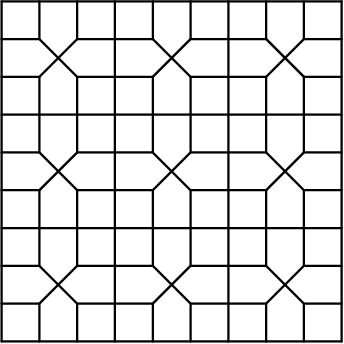
\includegraphics[height=5cm,page=1]{2021-07-10-figure-06}
\end{center}

\nopagebreak

\fbox{(A) $50$ \quad (B) $52$ \quad (C) $54$ \quad (D) $56$ \quad (E) $58$}

\begin{answer}
There are nine identical squares, so we can focus on a single square to calculate the percentage enclosed by pentagons. There are $4$ squares and $4$ pentagons, so we can focus on a single square and a single pentagon. A square is fully contained inside a pentagon, so we can immediately rule out $50$. It is also clear by inspection that a pentagon's extra area is exactly one-quarter of a square, that is $25\%$ more. The ratio is thus
\begin{align*}
\frac{125}{100+125} = \frac{125}{225} = \frac{5}{9} \approx 55.56
\end{align*}

Graphically, this corresponds to the shaded area in the figure:
\begin{center}
  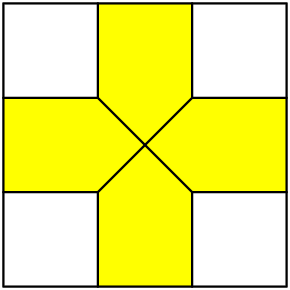
\includegraphics[height=3cm,page=1]{2021-07-10-figure-06b}
\end{center}
The square is itself divided into $9$ smaller squares, with the shaded area covering $5$ of those. 

\begin{empheq}[box={\mathbox[colback=white]}]{equation*}
    \approx 56
\end{empheq} 
\end{answer}
%%%%%%%%%%%%%%%%%%%%%%%%%%%%%%%%%%%%%%%%%%%%%%%%%%%%%%%%%%%%%%%%%%%%%%%%

\iftoggle{showAnswers}{\newpage}

%%%%%%%%%%%%%%%%%%%%%%%%%%%%%%%%%%%%%%%%%%%%%%%%%%%%%%%%%%%%%%%%%%%%%%%%
\subsection*{7.}

\nopagebreak

Let $A$, $M$, and $C$ be non-negative integers such that $A + M + C = 10$. What is the maximum value of $A \cdot M \cdot C + A \cdot M + M \cdot C + C \cdot A$?

\nopagebreak

\fbox{(A) $49$ \quad (B) $59$ \quad (C) $69$ \quad (D) $79$ \quad (E) $89$}

\begin{answer}
Since these are non-negative integers that sum to $10$, there aren't too many feasible triples, so we could realistically examine them all. For instance, it's clear that $(3,3,4)$ is a better choice than $(1,1,8)$. It's clear too that we can always do better than picking a $1$, that is $A,M,C$ can only be $2,3,4,5,6$. 

Suppose we knew one of the solutions and had to select the other two. In this case we would want to make the product of the two integers as large as possible. To see this, suppose we knew $C=1$ (of course, that's guaranteed to be wrong, but it conveniently eliminates $C$ from the expression so we can see more clearly the tradeoffs). We would now select $A$ and $M$ to maximize
\begin{align*}
& A \cdot M + A \cdot M + M + A \\
& \text{s.t}~ A + M = k
\end{align*}
where $k$ is some fixed constant (equal to $10-C=9$ in the case $C=1$), that is we would now select $A$ to maximize
\begin{align*}
2A(k-A)
\end{align*}
which is achieved for $A \approx k/2$. The same result holds for any given value of $C$. In general, to maximize the product $AMC$ for given $A+M+C$, we select $A,M,C$ as close to each other as possible. Since all the terms in the expression to be maximized are positive products of two or three of $A,M,C$, the principle is clear: make $A$, $M$, $C$ as close to each other as possible, given that $A+M+C=10$. We would select $A=M=C=10/3$ if it were allowed, but since only non-negative integers are allowed we select $(3,3,4)$, for a maximum of 
\begin{align*}
& A \cdot M \cdot C + A \cdot M + M \cdot C + C \cdot A \\
& = 3 \times 3 \times 4 + 3 \times 3 + 3 \times 4 + 4 \times 3 \\
& = 69
\end{align*}
\begin{empheq}[box={\mathbox[colback=white]}]{equation*}
    69
\end{empheq} 
\end{answer}
%%%%%%%%%%%%%%%%%%%%%%%%%%%%%%%%%%%%%%%%%%%%%%%%%%%%%%%%%%%%%%%%%%%%%%%%

\iftoggle{showAnswers}{\newpage}

%%%%%%%%%%%%%%%%%%%%%%%%%%%%%%%%%%%%%%%%%%%%%%%%%%%%%%%%%%%%%%%%%%%%%%%%
\subsection*{8.}

\nopagebreak

The mean, median, unique mode, and range of a collection of eight integers are all equal to $8$. The largest integer that can be an element of this collection is

\nopagebreak

\fbox{(A) $11$ \quad (B) $12$ \quad (C) $13$ \quad (D) $14$ \quad (E) $15$}

\textbf{Note:} The mode is the most frequent number, and the range is the difference between the lowest number and the highest number. For example, the mode of the numbers $2, 2, 7, 7, 7, 7, 13, 13, 13$ is $7$, and the range is $13-2=11$.

\begin{answer}
Since the mode is $8$, we must have at least two $8$s among the integers. Since the median is $8$, we must have three integers greater than $8$ and three smaller than $8$. Since the mean is $8$, we must have that the sum of the deviations from the mean are equal below and above $8$. Something like the following: $7-d,7,7,8,8,9,9,9+d$, for some $d$, checks all the boxes. Since the range must be $8$, that gives
\begin{align*}
(9+d)-(7-d) = 8
\implies d = 3
\end{align*}
and so the largest integer would be $9+3=12$. 

Can we improve on that? Clearly, replacing the $9$s by $8$s does not affect the mode and the median, while allowing us to increase the maximum. This change gives $7-d,7,7,8,8,8,8,11+d$. We can improve further with something like $7-d,7-d,7-d,8,8,9,9,11+3d$, for some $d$, since that allows us to increase the maximum. For the range to be $8$, $d$ must satisfy:
\begin{align*}
(11+3d)-(7-d) = 8
\implies d = 1
\end{align*}
and so the largest integer is $11+3=14$. 
\begin{empheq}[box={\mathbox[colback=white]}]{equation*}
    14
\end{empheq} 
(Note that if this last candidate solution hadn't divided evenly, we would have considered $7-d,7-d,7,8,8,9,9,11+2d$ instead.)
\end{answer}
%%%%%%%%%%%%%%%%%%%%%%%%%%%%%%%%%%%%%%%%%%%%%%%%%%%%%%%%%%%%%%%%%%%%%%%%

\iftoggle{showAnswers}{\newpage}

%%%%%%%%%%%%%%%%%%%%%%%%%%%%%%%%%%%%%%%%%%%%%%%%%%%%%%%%%%%%%%%%%%%%%%%%
\subsection*{9.}

\nopagebreak

A rectangular floor measures $a$ feet by $b$ feet, where $a$ and $b$ are positive integers with $b > a$. An artist paints a rectangle on the floor with the sides of the rectangle parallel to the sides of the floor. The unpainted part of the floor forms a border of width $1$ foot around the painted rectangle and occupies half the area of the entire floor. How many possibilities are there for the ordered pair $(a,b)$?

\nopagebreak

\fbox{(A) $1$ \quad (B) $2$ \quad (C) $3$ \quad (D) $4$ \quad (E) $5$}

\begin{answer}
The total area of the floor is $ab$. The painted area has dimensions $a-2$ and $b-2$ and area half of $ab$, so that $a$ and $b$ satisfy:
\begin{align*}
(a-2)(b-2) 
  & = \frac{ab}{2}
\end{align*}
To solve for positive integers $a, b$, we first develop the expression and then factor it by ``completing the rectangle'':
\begin{align*}
ab - 4a - 4b + 8 & = 0 \\
(a-4)(b-4) -16+8 & = 0 \\
(a-4)(b-4) & = 8 
\end{align*}
The following pairs satisfy the conditions: $(5,12)$ and $(6,8)$. That is two ordered pairs. 
\begin{empheq}[box={\mathbox[colback=white]}]{equation*}
    2
\end{empheq} 
\end{answer}
%%%%%%%%%%%%%%%%%%%%%%%%%%%%%%%%%%%%%%%%%%%%%%%%%%%%%%%%%%%%%%%%%%%%%%%%

\iftoggle{showAnswers}{\newpage}

%%%%%%%%%%%%%%%%%%%%%%%%%%%%%%%%%%%%%%%%%%%%%%%%%%%%%%%%%%%%%%%%%%%%%%%%
\subsection*{10.}

\nopagebreak

When $15$ is appended to a list of integers, the mean is increased by $2$. When $1$ is appended to the enlarged list, the mean of the enlarged list is decreased by $1$. How many integers were in the original list?

\nopagebreak

\fbox{(A) $4$ \quad (B) $5$ \quad (C) $6$ \quad (D) $7$ \quad (E) $8$}

\begin{answer}
Let $x_{k}$ denote the $n$ integers in the list. The conditions may be expressed as:
\begin{align*}
\frac{x_{1} + x_{2} + \ldots + x_{n} + 15}{n+1} 
  & = \frac{x_{1} + x_{2} + \ldots + x_{n}}{n} + 2 \\
\frac{x_{1} + x_{2} + \ldots + x_{n} + 15 + 1}{n+2} 
  & = \frac{x_{1} + x_{2} + \ldots + x_{n}}{n} + 2 - 1
\end{align*}
We want to solve for $n$, so we seek to eliminate the $x_{k}$s. To this effect, let $s$ denote their sum. The condition may now be written:
\begin{align*}
\frac{s + 15}{n+1} & = \frac{s}{n} + 2 \\
\frac{s + 15 + 1}{n+2} & = \frac{s}{n} + 2 - 1
\end{align*}
Remove the fractions by cross-multiplying:
\begin{align*}
n(s + 15) & = (n+1)(s+2n) \\
n(s + 16) & = (n+2)(s+n) 
\end{align*}
We notice that the $ns$ term on each side cancel out, so we develop and simplify:
\begin{align*}
2n^2 -13n + s  & = 0  \\
n^2 - 14n + 2s & = 0
\end{align*}
We can now eliminate $s$ and get an equation for $n$. Multiply the first equation by $2$ and subtract the second equation:
\begin{align*}
n^2 -4n = 0  
\implies
n = 4
\end{align*}
\begin{empheq}[box={\mathbox[colback=white]}]{equation*}
    4
\end{empheq} 
\end{answer}
%%%%%%%%%%%%%%%%%%%%%%%%%%%%%%%%%%%%%%%%%%%%%%%%%%%%%%%%%%%%%%%%%%%%%%%%

\end{document}
